%-----------------------------------------------------------------------------
% cabeçalho
%-----------------------------------------------------------------------------
\documentclass{beamer}

% para criar um documento para acompanhamento, comente a linha acima e
% descomente as linhas abaixo.
%\documentclass[handout]{beamer}
%\usepackage{pgfpages}
%\pgfpagesuselayout{4 on 1}[a4paper,border shrink=5mm]


% localização
\usepackage[utf8x]{inputenc}
\usepackage[brazil]{babel}
%\usepackage{abntex}

% embelezamento
\usepackage{amssymb,amsmath,amsfonts}
\numberwithin{equation}{section}
\usepackage{enumerate}
\usepackage{xspace}
%\usetheme{Goettingen} % <---- so com crane
%\usetheme{sidebar}   % <---- com crane fica bom
%\usecolortheme{crane} % <---- Goettingen com crane
\usepackage{colortbl}
\usepackage{url}
\usepackage{color}

% figuras
\usepackage{tikz}
\usetikzlibrary{arrows}

% Sumário no início de cada seção
\AtBeginSection[]
{
  \begin{frame}<beamer>{Estrutura da apresentação}
    \tableofcontents[currentsection]
  \end{frame}
}

% comandos
\definecolor{meuvermelho}{RGB}{200,40,40}
\definecolor{meuazul}{RGB}{40,40,140}
\newcommand{\enfase}[1]{{\color{meuvermelho}#1}}
\newcommand{\enfasel}[1]{{\color{meuazul}#1}}
\newcommand{\Pe}{{\color{meuazul}\ensuremath{P}}\xspace}
\newcommand{\Petil}{{\color{meuazul}\ensuremath{\tilde{P}}}\xspace}
\newcommand{\Ve}{{\color{meuvermelho}\ensuremath{V}}\xspace}
\newcommand{\inlet}{\emph{inlet}}
\newcommand{\inlets}{\emph{inlets}}
\newcommand{\outlet}{\emph{outlet}}
\newcommand{\outlets}{\emph{outlets}}
\newcommand{\Inlet}{\emph{Inlet}}
\newcommand{\Inlets}{\emph{Inlets}}
\newcommand{\Outlet}{\emph{Outlet}}
\newcommand{\Outlets}{\emph{Outlets}}


%-----------------------------------------------------------------------------
% Dados para o primeiro slide
%-----------------------------------------------------------------------------

\title
{Como escrever \emph{externals} em C para estender o Pure Data}

%\subtitle
%{}

\author
{Flávio Luiz Schiavoni\\
\footnotesize{fls@ime.usp.br}}

\institute
[Universidade de São Paulo]
{
  Departamento de Ciência da Computação\\
  Instituto de Matemática e Estatística \\
  Universidade de São Paulo
}

\date{\today}


%-----------------------------------------------------------------------------
% Documento
%-----------------------------------------------------------------------------
\begin{document}

\begin{frame}
  \titlepage
\end{frame}

%-----------------------------------------------------------------------------
\begin{frame}{Objetivo da apresentação}

Introduzir à escrita de \emph{externals} para Pure Data, considerando:
\begin{itemize}
  \item Como escrever.
  \item Como compilar.
  \item Exemplos.
\end{itemize}
\end{frame}

%-----------------------------------------------------------------------------
\begin{frame}{Estrutura da apresentação}
  \tableofcontents
\end{frame}

% Since this a solution template for a generic talk, very little can
% be said about how it should be structured. However, the talk length
% of between 15min and 45min and the theme suggest that you stick to
% the following rules:  

% - Exactly two or three sections (other than the summary).
% - At *most* three subsections per section.
% - Talk about 30s to 2min per frame. So there should be between about
%   15 and 30 frames, all told.

%-----------------------------------------------------------------------------
% Seções
%-----------------------------------------------------------------------------
\section{Introdução}

\begin{frame}{Pure Data}
\begin{figure}
\centering
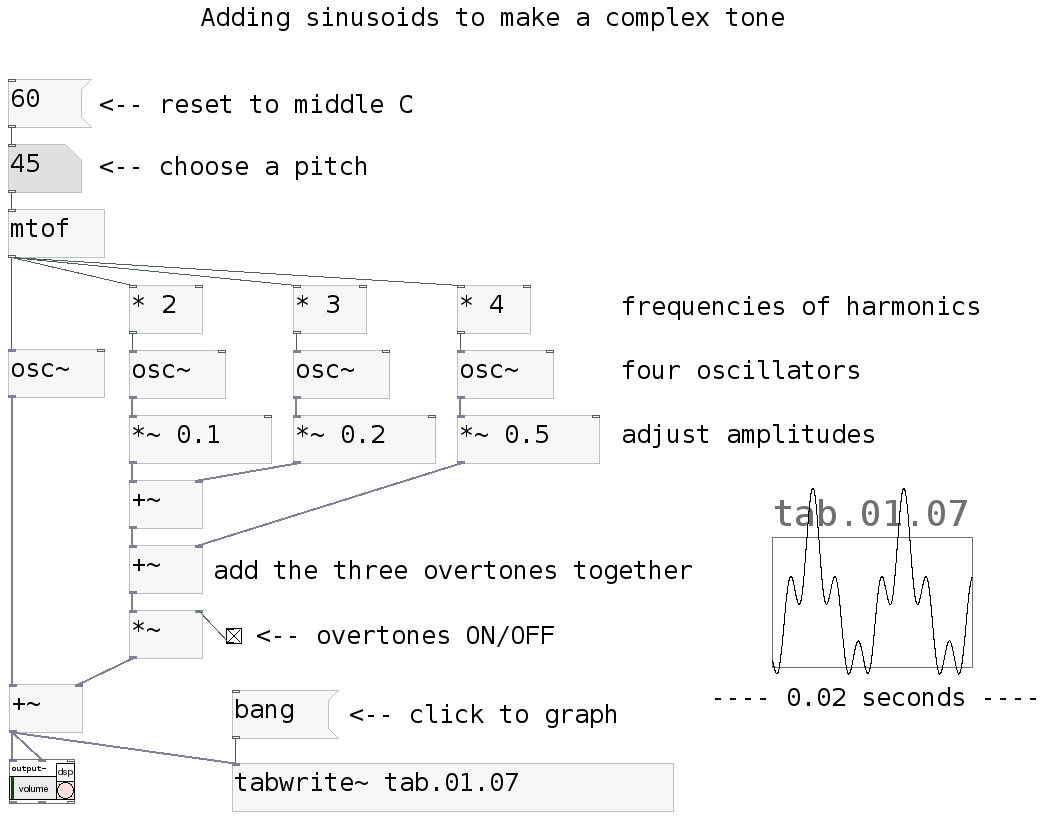
\includegraphics[width=0.7\textwidth]{../images/pd-facil}
%\caption{Um Arduino.}
\end{figure}
\end{frame}


\begin{frame}{Formas de estender o Pure Data}
Existem algumas formas de estender as funcionalidades do Pure Data:
\begin{itemize}
\item Subpatches.
\item \enfasel{Externals}.
\item Alterações no código-fonte.
\end{itemize}
\pause
\vspace{1em}
Este seminário trata da extensão do Pure Data através da criação de
\externals em C.
\end{frame}


\begin{frame}[fragile]{Organização do código e compilação}
\begin{itemize}
\item \texttt{meu-external.c}: \\
  \hspace{1em}\texttt{\#include <m\_pd.h>}
\item Compilação: \\
  \hspace{1em}\texttt{meu-external.c} $\rightarrow$ \texttt{meu-external.pd\_linux} \\
  \hspace{1em}\texttt{meu-external.c} $\rightarrow$ \texttt{meu-external.pd\_irix5} \\
  \hspace{1em}\texttt{meu-external.c} $\rightarrow$ \texttt{meu-external.pd\_darwin} \\
  \hspace{1em}\texttt{meu-external.c} $\rightarrow$ \texttt{meu-external.dll} \\
\end{itemize}
\end{frame}


\begin{frame}[fragile]{Compilação}
\begin{lstlisting}
EXTNAME=meu-external
cc -DPD -fPIC -Wall -o ${EXTNAME}.o -c ${EXTNAME}.c
ld -shared -lc -lm -o ${EXTNAME}.pd_linux ${EXTNAME}.o
rm ${EXTNAME}.o
\end{lstlisting}
O Pure Data procura por objetos com nomes diferentes em cada sistema:
\begin{itemize}
  \item \texttt{meu-external.\enfase{pd\_linux}} (GNU/Linux).
  \item \texttt{meu-external.\enfase{pd\_irix5}} (Irix 5).
  \item \texttt{meu-external.\enfase{pd\_darwin}} (Mac OS X).
  \item \texttt{meu-external.\enfase{dll}} (MS Windows).
\end{itemize}
\end{frame}


\begin{frame}[fragile]{Arquivos de ajuda}
Um arquivo de ajuda é um patch do Pure Data com:
\begin{itemize}
\item Um nome informativo: \texttt{meu-external\enfase{-help}.pd}.
\item Instruções de uso.
\item Exemplos de utilização.
\end{itemize}
\vspace{2em}
A seguinte função associa um arquivo de ajuda a uma classe de \external:
\begin{lstlisting}
class_sethelpsymbol(meu-external_class, gensym("meu-external_class-help"));
\end{lstlisting}
\end{frame}


\begin{frame}{Utilizando \externals}
Passos para utilizar um \external no Pure Data:
\begin{enumerate}
\item Escreva um arquivo \texttt{.c} com as funções, classes e métodos.
\item Compile o código-fonte para criar uma biblioteca compartilhada.
\item Informe ao Pure Data o caminho para o \external através de uma das
opções abaixo:
  \begin{enumerate}
    \item Na linha de comando, utilize a opção \enfasel{\texttt{-path
    <caminho>}}.
    \item Na interface gráfica, acesse a opção \enfasel{\texttt{File} $\rightarrow$
    \texttt{Path...}}.
    \item Na criação do objeto, insira o caminho completo (relativou ou
    absoluto) para o objeto do \external.
  \end{enumerate}
\item Crie um objeto com o nome do arquivo do \external, sem a extensão.
\end{enumerate}
\end{frame}


\begin{frame}{Utilizando \externals}
\begin{figure}[h!]
  \centering
  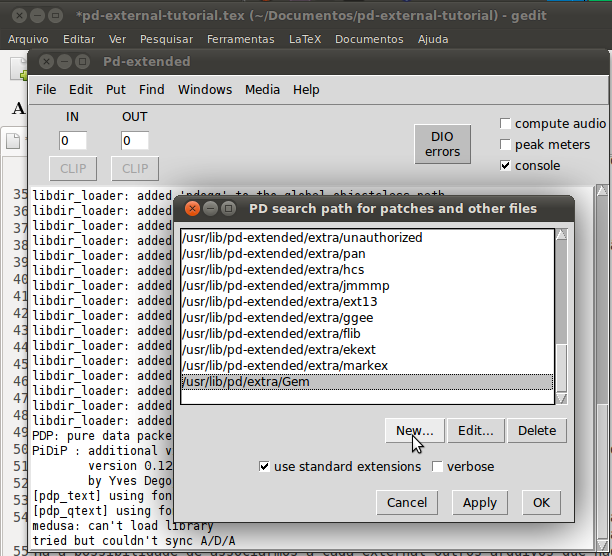
\includegraphics[width=0.7\textwidth]{../images/path}
  \caption{Adicionando o diretório de um \external ao caminho de busca do Pure Data.}
  \label{fig:search-path}
\end{figure}
\begin{itemize}
\item
\end{itemize}
\end{frame}

\section{Conclusão}

\begin{frame}{Referências}
\begin{itemize}
\item Repositório oficial de externals do Pure Data\footnote{http://pure-data.svn.sourceforge.net/viewvc/pure-data/trunk/externals}.
\item Tutorial do IOHannes\footnote{http://iem.at/pd/externals-HOWTO/pd-externals-HOWTO.pdf}.
\item Código fonte do Pure Data\footnote{http://pure-data.git.sourceforge.net/}.
\end{itemize}
\end{frame}


\begin{frame}{Dúvidas?}
{Obrigado!}
\texttt{http://www.ime.usp.br/$\sim$fls}

\texttt{https://github.com/flschiavoni/pd-external-tutorial}

\texttt{http://compmus.ime.usp.br/}
\end{frame}



\end{document}
